%!TEX root = pfc-memoria.tex
%!TEX encoding = UTF-8 Unicode

\chapter{Introducción}

\epigraph{``Los sentimientos y las emociones son el lenguaje universal que debe ser honrado. Son la expresión auténtica de quiénes somos.''}{\textsc{Judith Wright} (1915--2000)}

Durante la carrera tenemos asignaturas que tratan sobre procesamiento de lenguajes, pero siempre lenguajes formales. El lenguaje natural es mucho más complejo y ambiguo, y difícil de procesar.

\begin{definition}[NLP]\index{NLP}\index{procesamiento del lenguaje natural}\index{natural language processing@\emph{natural language processing}}
El procesamiento de lenguaje natural (PLN, o NLP del inglés \emph{Natural Language Processing}) es el campo de ciencias de la computación, inteligencia artificial y lingüística que estudia las interacciones entre las computadoras y el lenguaje humano \citep[Procesamiento de lenguajes naturales]{wikipedia-es}.
\end{definition}

Para conseguir procesar el lenguaje natural de forma eficiente se debe proveer a las computadoras de herramientas para comprender el conocimiento humano expresado en lenguaje natural (voz o texto, principalmente), y saber representarlo. En regla general, el lenguaje natural es abierto a interpretaciones, de manera que los resultados de estas técnicas no pueden ser 100\% exactos siempre, y aceptaremos resultados parciales y aproximaciones.

Con la aparición de la denominada \nombrebf{Web 2.0}, las páginas dinámicas, y los gestores de contenido web, los consumidores de información (usuarios o visitantes de páginas web) son también productores de la información. Estos usuarios producen en su mayoría contenido de tipo texto, obviamente en lenguaje entendible por otros humanos, con poca capacidad para el \emph{software} de realizar cualquier cálculo, extracción, comprensión, o modificación al mismo en documentos sin una estructura formalizada previa ni preparados para ser consumido por la máquinas. En el estudio de \citet{Hilbert2011}, se estima cuál es la capacidad global de información generada, en su tramo analógico y digital a lo largo del tiempo, observando una explosión digital a partir del año 2002 (\autoref{fig:InfoGrowth}).

De esta manera, ha suscitado un mayor interés por la comunidad científica en aprovechar esa vasta cantidad de información disponible para comprender los datos y extraer información útil resumida de ellos y con alguna aplicabilidad, en las llamadas tareas de \nombrebf{minería de datos} (en inglés: \emph{data mining}).\index{minería!de datos}\index{data mining}

En el caso del análisis de textos: \nombrebf{minería de textos}.\index{minería!de textos}\index{text mining}

\begin{landscape}
\begin{figure}[htbp]
\centering
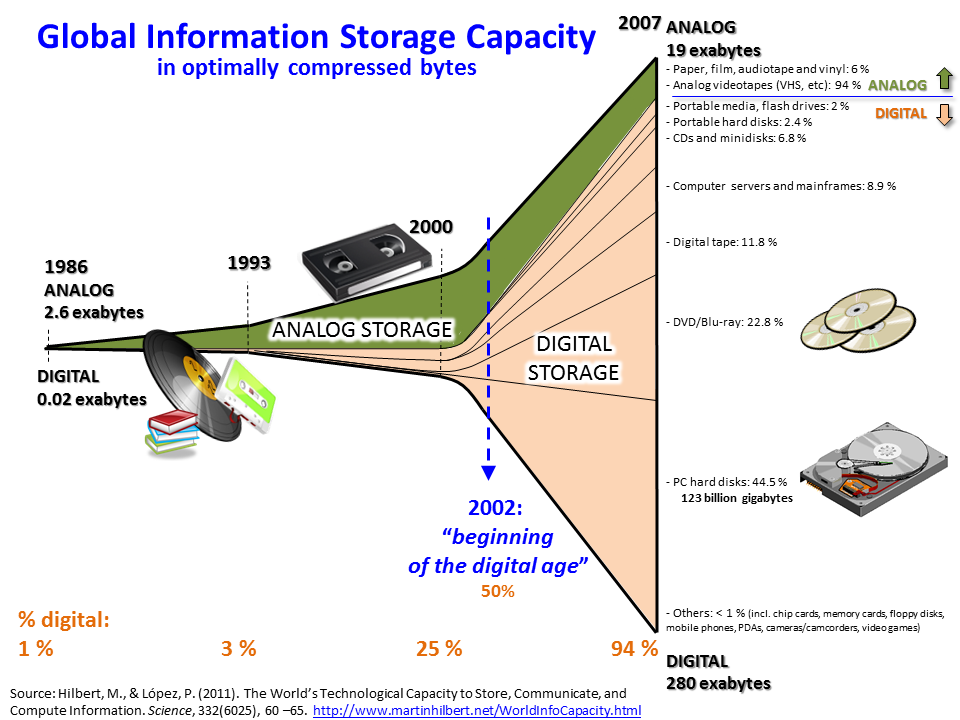
\includegraphics[height=0.85\textwidth]{Hilbert-InfoGrowth}
\caption[Explosión de información digital]{Gracias a la \nombrebf{explosión de información digital}, existe actualmente gran cantidad de información disponible para extraer el conocimiento humano, inclusive el lenguaje natural, de manera automática, por las máquinas \citep{Hilbert2011}. \\
{\footnotesize ``Hilbert InfoGrowth'' by Myworkforwiki - Own work. Licensed under CC BY-SA 3.0 via Wikimedia Commons - \url{https://commons.wikimedia.org/wiki/File:Hilbert_InfoGrowth.png\#/media/File:Hilbert_InfoGrowth.png}}}
\label{fig:InfoGrowth}
\end{figure}
\end{landscape}

\section{Sentimiento o polaridad de las opiniones}

En los documentos de tipo crítico, o comentarios de opinión acerca de una película, un artículo o un servicio, la información que se extrae de su lectura es si la película, el artículo o el servicio le ha parecido bueno o malo. A esto se le llama la \nombrebf{polaridad del sentimiento}\index{polaridad!sentimiento}\index{sentimiento}\index{polaridad} (o simplemente sentimiento) de la crítica. Se puede ver un ejemplo de escala de valoración de esta polaridad (con varias graduaciones entre negativo y positivo) en la \autoref{fig:tramos-polaridad}.

\begin{figure}[htbp]
\centering
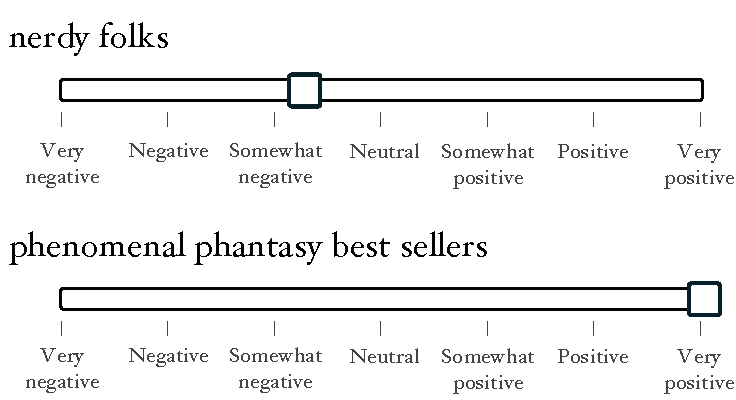
\includegraphics[height=5.5cm]{tramos-polaridad}
\caption[Escala de valoración del sentimiento en Penn Sentiment Treebank]{Escala de valoración del sentimiento empleada en el proyecto Penn Sentiment Treebank de la Universidad de Pennsylvania \citep{Socher2014}}
\label{fig:tramos-polaridad}
\end{figure}


En las páginas dedicadas a opiniones de productos en general como \nombre{Ciao!}\footnote{\url{http://www.ciao.es/}}, o más específicamente para críticas de cine como \nombre{FilmAffinity}\footnote{\url{http://www.filmaffinity.com/}}, se suele proporcionar al usuario un formulario para introducir un texto con su crítica, y además un elemento para que etiquete su valoración, bien en una escala de puntuación o bien mediante estrellitas.

\begin{figure}[htbp]
\centering
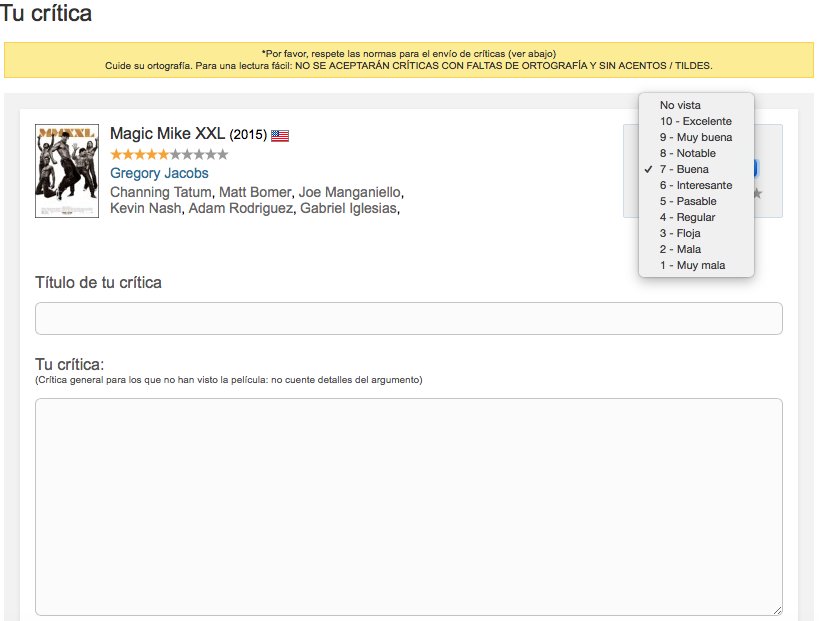
\includegraphics[width=\textwidth]{filmaffinity}
\caption[Introducción de la valoración en FilmAffinity]{En \href{http://www.filmaffinity.com/}{FilmAffinity} han optado por el desplegable de 1 a 10 puntos etiquetados para introducir la valoración}
\label{fig:filmaffinity}
\end{figure}

\begin{figure}[htbp]
\centering
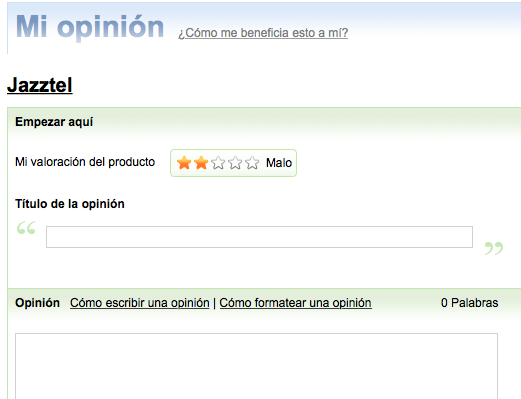
\includegraphics[width=0.7\textwidth]{ciao}
\caption[Introducción de la valoración en ciao.es]{Introducción de la valoración en \href{http://www.ciao.es/}{Ciao!}, con estrellitas}
\label{fig:ciao}
\end{figure}

En este tipo de documentos es fácil determinar cuál es la polaridad del texto de la crítica, pues tenemos disponible además un campo de tipo numérico o enumerado (numérico en el sentido de ser inmediatamente procesable por la máquina, sin mayor tratamiento que quizás un cambio de escala o conversión de tipo entero a coma flotante) con la valoración, y podemos asociar valoraciones altas con polaridad buena o muy buena, y las valoraciones bajas con polaridad mala o muy mala. Las valoraciones medias se asociarían a comentarios cuya polaridad del sentimiento será neutra.

\section{Motivación}

Con el amplio uso de las plataformas de twitter y Facebook, los consumidores de productos y servicios pueden criticar abiertamente mediante un comentario a las marcas de las empresas cuyos productos han gustado o no (pero sin un campo específico para la valoración). En la vida virtual, al igual en la vida real, las personas comentamos con nuestros familiares y amigos, y recomendamos o no recomendamos estos productos, contribuyendo con nuestras experiencias a mejorar o empeorar la \nombrebf{reputación de la marca.}\index{reputación!de marca}

Twitter se ha consolidado de esta manera como una forma digital de boca a boca \citep{Jansen2009}, pero con mayores posibilidades de alcanzar un gran impacto (o \nombrebf{viralidad}\index{viralidad}) al distribuirse mediante la red global de Internet, y potencialmente llegar a gran cantidad de público. Es más, por nuestra naturaleza, tendemos a reproducir la mala publicidad de un compañía con mayor asiduidad que la buena publicidad, por eso las empresas deben estar presentes en las redes sociales y monitorear su \nombrebf{reputación online}\index{reputación!online} \citep{Leiva2012} o \emph{e-reputación}.

\begin{example}[Crisis de reputación de Zara (2014)]
En 2014, la marca del grupo Inditex ponía a la venta una camiseta rayada y con una estrella de sheriff en el pecho. Nadie podía imaginar la cantidad de comentarios negativos que se publicaron sobre la camiseta y sobre Zara a partir de una noticia en el diario israelí \nombre{Haaretz}: ``Striping resemblance: Zara tee looks like Holocaust garb'',\footnote{\url{http://www.haaretz.com/jewish-world/jewish-world-news/1.612710}} comparando el diseño de la misma con el uniforme que llevaban los judíos durante el holocausto nazi (\autoref{fig:zara-camiseta}).

\begin{figure}[htbp]
\centering
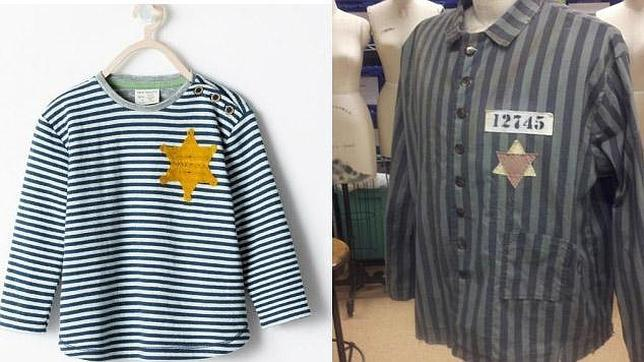
\includegraphics[width=0.7\textwidth]{zara-camiseta}
\caption[Diseño de la camiseta de Zara, y uniforme judío en el holocausto]{Diseño de la camiseta de Zara, y uniforme judío usado en el holocausto\footnotemark}
\label{fig:zara-camiseta}
\end{figure}
\footnotetext{Ejemplo extraído de \url{http://blog.prodware.es/crisis-de-reputacion-online-en-2014/}. En el artículo también se comentan otros casos de errores en la gestión de crisis de reputación online, sufridos por las marcas Garnier y Heineken.}

\newpage
Algunos de los mensajes que se publicaron en aquel momento fueron:\footnote{\url{https://storify.com/almas2205/twitter-users-express-outrage-over-zara-t-shirts-f}}
\begin{itemize}
\item Nathalie Rothschild (@n\_rothschild) 10:17 AM - 27 Aug 2014 \\ --- What were the designers thinking @ZARA ? \url{http://t.co/SukupXR3XN}
\item Carolina Farraj (@Carolinafarraj) 1:23 PM - 27 Aug 2014 \\ --- Hey @ZARA ! What the ell is wrong with you?!
\item Ciaran Walsh (@kowalshki) 11:51 AM - 27 Aug 2014 \\ --- Complete fashion fail by ZARA. \url{http://t.co/yGdUa5tf5b}
\item Linton Kwesi Johnson (@LKwesiJ) 10:36 AM - 27 Aug 2014 \\ --- .@n\_rothschild I'll just presume the folks at @ZARA have no historical understanding or knowledge whatsoever. Not sure what else to think.
\end{itemize}

El revuelo causado por la mala crítica en las redes sociales obligó a la compañía a retirar el producto y pedir disculpas públicamente.\footnote{\url{http://www.independent.co.uk/life-style/fashion/zara-apologises-for-striped-holocaust-shirt-with-yellow-star-after-twitter-backlash-9693963.html}}

Aun con todo eso, la delegación israelita de Zara tuvo la ocurrencia ---con una evidente carencia de sensibilidad--- de expresar la disculpa excusándose en que la línea de la colección estaba inspirada en las películas del salvaje oeste, y que las ``camisetas serán exterminadas'', algo que obviamente sirvió para avivar aún más la polémica.\footnote{\url{http://972mag.com/nstt_feeditem/zara-apologizes-says-yellow-star-shirts-will-be-exterminated/}}
\end{example}

Es por eso que este trabajo se enfoca en cómo procesar los textos para obtener las reglas necesarias para determinar si un comentario es o no positivo, y realizar una aplicación para comprobar su eficacia con un caso concreto. El proyecto se utilizará para su aplicación en la participación en el concurso de \nombre{kaggle:} ``Sentiment Analysis on Movie Reviews'',\footnote{\url{https://www.kaggle.com/c/sentiment-analysis-on-movie-reviews}} sobre la base de datos de críticas de cine de \nombre{Rotten Tomatoes}.\footnote{\url{http://www.rottentomatoes.com}}

\section{Estructura de la memoria}

Aparte de la \fullref{part:introduccion-objetivos}, la memoria del proyecto se divide en dos partes principalmente:
\begin{itemize}
\item La \fullref{part:investigacion-estudio} es un estudio de investigación sobre algunas de las técnicas de procesamiento de lenguaje natural, consolidadas y experimentales; y además de los métodos de aprendizaje automático para la fase de entrenamiento.
\item En la \fullref{part:desarrollo-proyecto} se detalla el calendario, análisis, desarrollo e implementación del proyecto software.
\end{itemize}

La última \fullref{part:apendices} contiene el manual de usuario y la bibliografía y referencias utilizadas; así como los índices de tablas, figuras, códigos y conceptos.
